\documentclass[10pt,a4paper]{article}
\usepackage[utf8]{inputenc}
\usepackage[magyar]{babel}
\usepackage[T1]{fontenc}
\usepackage{amsmath}
\usepackage{amsfonts}
\usepackage{amssymb}
\usepackage{graphicx}
\begin{document}
\title{Méréstechnika laboratórium II 15. jegyzőkönyv}
\author{Koncz István Márton}
\date{\today}
\maketitle
\newpage

\section{15. sz. laboratóriumi mérés}
	Mérés dátuma:\date{2016.09.27}
	\subsection{A mérés célja}
	Kapuzással és impulzusszámlálással dolgozó digitális frekvencia- és időmérő
működési elvének és működésének modellen történő bemutatása az alapvető
üzemmódokban. A kapcsolást alkotó áramkörök vizsgálata.

	\subsection{Mérési feladatok}
		\subsubsection{Az Nx számláló számlálási bizonytalanságának mérése}
		Állítson be a függvénygenerátoron kb. 15Hz-es négyszög-jelet! Válasszon a
mérőpanel frekvenciamérő üzemmódjában 10MHz-es méréshatárt és mérje
meg a jel frekvenciáját!
		$$$$ $$$$ $$$$ $$$$ $$$$ $$$$
		\subsubsection{Közvetlen frekvenciamérés}
		Oszcilloszkóp segítségével állítson be a függvénygenerátor kimenetén
négyszögjelet, a pozitív szint 3 V, a negatív szint 0 V legyen!
		\\\\
		Mérendő objektum:
		\begin{figure}[hbtp]
		\centering
		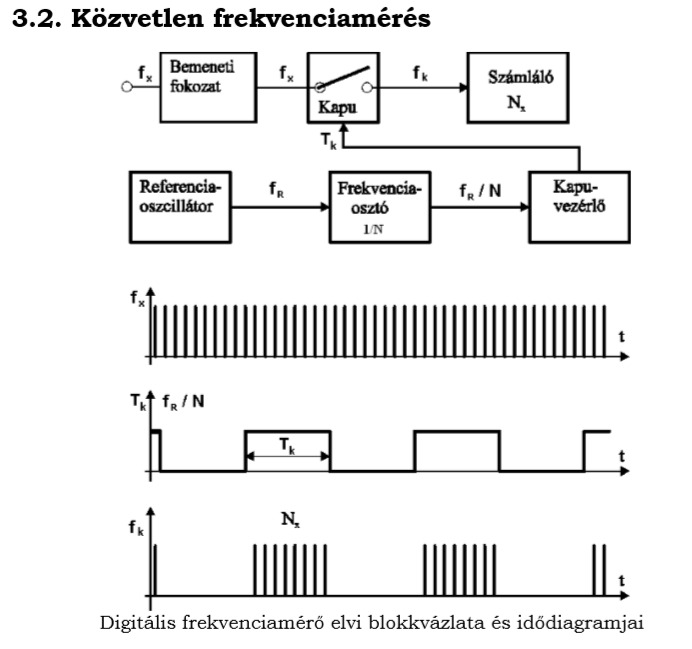
\includegraphics[scale=0.3]{teljes/kozv_frekvencia.png}
		\caption{}
		\end{figure}
		\newpage\begin{tabular}{|c|c|c|c|c|c|c|}
		\hline 
		f[Hz] & 10 & $10^2$ & $10^3$ & $10^4$ & $10^5$ & $10^6$ \\ 
		\hline 
		Nx &  &  &  &  &  &  \\ 
		\hline 
		$h_{fx}$ &  &  &  &  &  &  \\ 
		\hline 
		\end{tabular} 
		$$h_{fx} = h_{fR} + \frac{1}{Nx}; h_{fR} = $$
		$$Mode=FREQ; RANGE=10000 \frac{kHz}{ms}$$
		RANGE kapcsoló 3 állásának mérése:\\\\
		\begin{tabular}{|c|c|c|c|}
		\hline 
		RANGE & 100 kHz & 1000 kHz & 10000 kHz \\ 
		\hline 
		Nx &  &  &  \\ 
		\hline 
		$h_{fX}$ &  &  &  \\ 
		\hline 
		\end{tabular} 
		\\\\ $$$$
		\subsubsection{Periódusidőmérésen alapuló frekvenciamérés}
		Oszcilloszkóp segítségével állítson be a függvénygenerátor kimenetén
négyszögjelet, a pozitív szint 3 V, a negatív szint 0 V legyen!
		\\\\
		\begin{tabular}{|c|c|c|c|c|c|c|}
		\hline 
		f[Hz] & 1 & 10 & 100 & $10^3$ & $10^4$ & $10^5$ \\ 
		\hline 
		Nx &  &  &  &  &  &  \\ 
		\hline 
		$h_{fx}$ &  &  &  &  &  &  \\ 
		\hline 
		\end{tabular} 
		$$h_{Tx} = h_{fR} + \frac{1}{Nx}; h_{fR} = $$
		$$Mode=FREQ; RANGE=10000 \frac{kHz}{ms}$$
		RANGE kapcsoló 3 állásának mérése:\\\\
		\begin{tabular}{|c|c|c|c|}
		\hline 
		RANGE & 100 ms & 1000 ms & 10000 ms \\ 
		\hline 
		Nx &  &  &  \\ 
		\hline 
		$h_{fX}$ &  &  &  \\ 
		\hline 
		\end{tabular} 
		\\\\ $$$$ $$$$ $$$$
		\subsubsection{Időintervallum mérés}
		Oszcilloszkóp segítségével állítson be a függvénygenerátor kimenetén
impulzus jelalakot, a pozitív szint $3 V$, a negatív szint $0 V$, a kitöltési tényező $60 \%$ legyen! Az impulzus jelalak kiválasztása esetén az offset
potencióméterrel lehet a jel kitöltési tényezőjét állítani.\\\\
Állítson be a generátoron $1 kHz$ frekvenciát csatlakoztassa a 3 számú
mérőpanel $CH1$-es bemenetére. Állítsa a $MODE$ kapcsolót a $TIME$
állásban, a $RANGE$ kapcsolóval pedig állítsa be a maximális felbontást.
Mérje meg az impulzus szélességet!\\\\ \\\\ \\\\ \\\\


\end{document}